%\documentclass[preview, border=5mm]{standalone}
\documentclass[a3paper]{slides}

\usepackage[margin=2cm]{geometry}

% for the \xintFor***
\usepackage{xinttools} 
\usepackage{tikz}
\usetikzlibrary{calc,backgrounds}
\makeatletter
\newcommand\store[6][\x]{%
  % #1 = dummy variable
  % #2 = variable to store the list
  % #3 = expression
  % #4 = expression to store (with \pgfmathresult) and possibly #1
  % #5 = start point
  % #6 = end point
  \gdef\store@temp{\@gobble}%
  \foreach #1 in {#5,...,#6}{\pgfmathparse{#3}\xdef\store@temp{\store@temp,#4}}%
  \let#2=\store@temp
}
\makeatother


% playing role of infinity (should be < .25\maxdimen)
\def\bigLen{20cm}

% define the "half plane" to be clipped (#1 = half the distance between cells)
\tikzset{
  half plane/.style={
    to path={
       ($(\tikztostart)!.5!(\tikztotarget)!#1!(\tikztotarget)!\bigLen!90:(\tikztotarget)$)
    -- ($(\tikztostart)!.5!(\tikztotarget)!#1!(\tikztotarget)!\bigLen!-90:(\tikztotarget)$)
    -- ([turn]0,2*\bigLen) -- ([turn]0,2*\bigLen) -- cycle
    }
  },
  half plane/.default={2pt},
  conector/.style={
    to path={
       (\tikztostart)
    --(\tikztotarget)
    -- cycle
    }
  },
  conector/.default={2pt}
}

% random points are in [-\maxX,\maxY]x[-\maxX,\maxY]
%\def\maxX{ 13.85 }
\def\maxX{ \textwidth  * 0.5 }
\def\maxY{ \maxX * 1.44  }


% number of random points
\def\puntosCantidad{10} 
\def\paso{8}

\def\radio{10}
\def\centro{0}

\begin{document}

  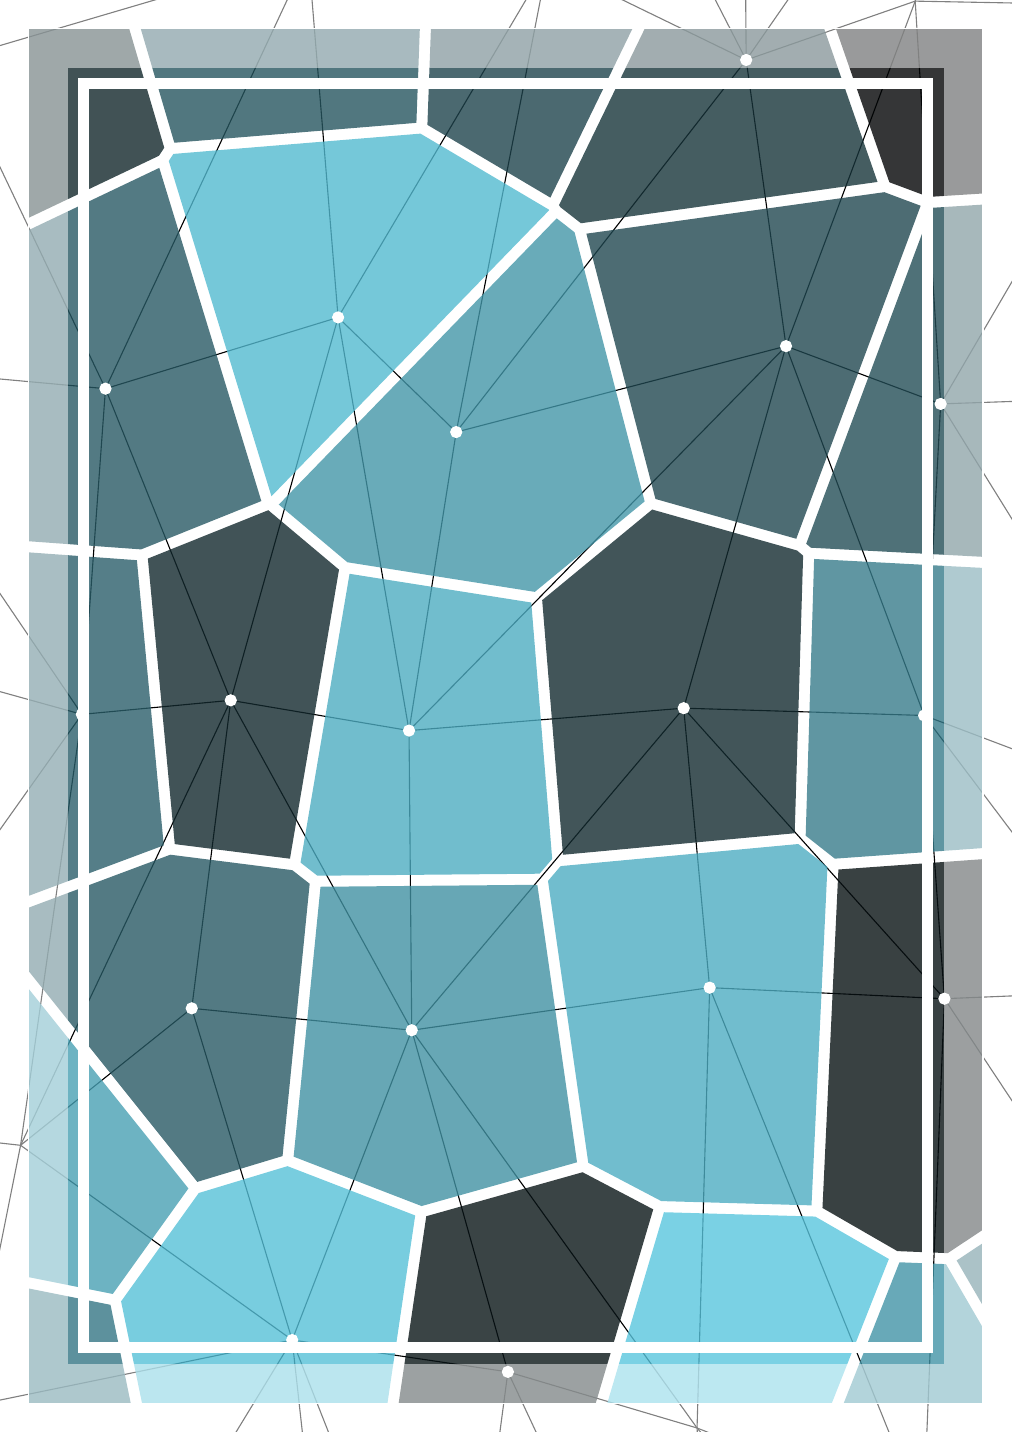
\begin{tikzpicture}
    %\draw (-\maxX,0) -- ( \maxX,0 );
    %\draw (0,-\maxY) -- ( 0,\maxY );

    % \pgfmathsetseed{1908}

    % Posicionar Puntos
    \def\cuenta{1}
    \gdef\puntos{}
    %\def\putos{}
    \xintFor* #1 in { \xintSeq {1}{\puntosCantidad} } \do{

      \def\grado{ \cuenta  }
      \edef\cuenta{\cuenta + \paso}

      \pgfmathsetmacro{\puntoX}{
        \centro 
        + ( \radio * cos( \grado ) )
        + ( rand ) 
      } 

      % random x in [-.9\maxY,.9\maxY]
      \pgfmathsetmacro{\puntoY}{ 
        \centro  
        + ( \radio * sin( \grado ) ) 
        + (rand )
      } 

      % stock the random point
     % \edef\puntos{\puntos, ( \puntoX, \puntoY )} 
    }

   %\store[\pepe]{\puntos}{rand}{(\pepe,\pepe)}{-10}{10}

   %\show\puntos


    \def\half{3}
    \foreach \i [evaluate={\ii=int(\i-1);}] in {-\half,...,\half}{
      \foreach \j [evaluate={\jj=int(\j-1);}] in {-\half,...,\half}{

	\pgfmathsetmacro{\radius}{ .5 + rnd }
	\pgfmathsetmacro{\angle}{ rand * 180 }
	\pgfmathsetmacro{\espacio}{ 3 }

        \coordinate [shift={( \i*\espacio, \j*\espacio*1.5 )}] (n-\i-\j) at ( \angle : \radius );

	\pgfmathsetmacro{\X}{(\i*\espacio) + \radius * cos(\angle) }
	\pgfmathsetmacro{\Y}{(\j*\espacio*1.5) + \radius * sin(\angle) }
	\xdef\puntos{\puntos, (\X,\Y) } 

          \ifnum\i> -\half
            \draw (n-\i-\j) -- (n-\ii-\j);
          \fi
          \ifnum\j>-\half
            \draw  (n-\i-\j) -- (n-\i-\jj);
            \ifnum\i>-\half
              \pgfmathparse{int(rnd>.5)}
              \ifnum\pgfmathresult=0
                \draw (n-\i-\j) -- (n-\ii-\jj);
              \else%
                \draw (n-\ii-\j) -- (n-\i-\jj);
              \fi%
            \fi
          \fi
    
      }
    }
    % draw the points and their cells
    \xintForpair #1#2 in \puntos \do{
      \edef\puntoA{#1,#2}

      \begin{scope}
        \xintForpair \#3#4 in \puntos \do{
          \edef\puntoB{#3,#4}

          % check if (#1,#2) == (#3,#4) 
          \ifx\puntoA\puntoB\relax 
            \tikzstyle{myClip}=[];
          \else
            \tikzstyle{myClip}=[clip ];
          \fi;
          \path [myClip] (#3,#4) to [half plane] (#1,#2);
        }
        % last clip
        \clip (-\maxX,-\maxY) rectangle (\maxX,\maxY); 

        \pgfmathsetmacro{\randSat}{ rnd }
        \definecolor{randcolor}{hsb}{ .53, .6, \randSat,  }
        % fill the cell with random color
        \fill[randcolor, opacity=.8 ] (#1,#2) circle (14*\bigLen); 
        % and draw the point
        \fill[draw=white,fill=white] (#1,#2) circle (2pt); 
      \end{scope}

    }

    \draw[draw=white,draw=white,line width=4pt] 
	  ({-\maxX + 20 },{-\maxY + 20 })
	  rectangle 
	  ({\maxX - 20	},{\maxY - 20 });
    \draw[draw=white,draw opacity=.5,line width=1cm] 
	  ({-\maxX },{-\maxY }) 
	  rectangle 
	  ({\maxX },{\maxY });

    \pgfresetboundingbox
	  \draw[draw=white] (-\maxX,-\maxY) rectangle (\maxX,\maxY );

  \end{tikzpicture}

\end{document}

